% https://github.com/andres-erbsen/trkuur
\documentclass[]{trkuur}
\input{preamble.trk.tex}

% Ingliskeelse teksti eristamine
\let\eng\emph
% Teksti seas oleva rogrammikoodi eristamine
\let\enp\eng
%\let\enp\texttt

\usepackage{amsmath}
\newcommand{\argmax}{\operatornamewithlimits{argmax}}

\addbibresource{mlmail.bib}
\title{Masinõppe kasutamine \\ oluliste kirjade tuvastamiseks}
\author{Andres Erbsen}
\klass{11c}
\juhendaja{tehnikamagister Inga Petuhhov \\ Konsultant: TÜ doktorant Konstantin Tretjakov}

\begin{document}


\maketitle
\tableofcontents

\addchap{Sissejuhatus}

Käesolev uurimistöö käsitleb kindlale isikule oluliste e-kirjade automaatset ja sõltumatut
äratundmist talle saabuvate kirjade hulgast. Küsimus püsib aktuaalne põhiliselt
olemasolevate lahenduste puuduste tõttu. Saatjapoolne kirja olulisuse hindamine
on harva abiks, kuna eeldab saatja adekvaatsust ja viitsimist sellega
tegelemiseks. Näide autori postkastist: isegi ainult mitte spämmiks loetud
kirjade hulgas olid neljateistkümnest sellel viisil oluliseks märgitud kirjast
ainult kaks ka saaja hinnangul olulised. Samuti ei ole lootust, et oleks olemas
üldine reegel --- inimeste huvid on erinevad.

Sama teemat on viimaste aastate jooksul korduvalt uuritud, kuid erinevate
eelduste ja eesmärkidega. Shinjae Yoo uurimistöö aastast 2010 keskendub
meiliside täpsele modelleerimisele, saavutades seeläbi palju detailsema
tulemuse automaatsel klassifitseerimisel \autocite[2]{SYoo2010}. Samuti avas käesoleva 
töö valmimise ajal Google oma meiliteenuse juures võimaluse saadud
kirjade olulisuse hindamiseks, kuid erinevalt käesolevast või Yoo poolt
läbi viidud uurimusest on see lahendatud lähtuvalt eeldusest, et hinnangu
andmiseks on kasutatavad ka teiste kasutajate andmed ja täpsem ülevaade kasutajate tegevustest kirjade lugemisel \autocite[1]{PrInboxML}. Nii Google kui
Yoo ootavad kasutajapoolset aktiivsust kirjade olulisuse märkimisel
või nende vastavalt sildistamisel, see lisatöö vähendab oluliselt kirjeldatud
lahenduste kasulikkust.

Teema valik oli ajendatud eelkõige soovist kirjeldatud olukorda muuta. 
Hüpoteesiks on väide, et analoogiliselt rämpsposti tuvastamisele
on võimalik arvutil olemasolevate masinõppemeetodite abil ära tunda olulisi kirju, kasutades
selleks ainult kasutaja kirjakastis loomulikult leiduvat infot.
Eesmärk on selgitada välja, kui tulemuslik on selline klassifitseerimine,
võrrelda erinevate klassifitseerijate sobivust selleks konkreetseks ülesandeks
ja luua minimaalne rakendus toimuva demonstreerimiseks.

Kasutusel olid kas peamist meetodit.
Esmalt e-kirjade analüüsimine võimalike olulisusega
seotud tunnuste leidmiseks.
Teiseks on loodud programm, mis nende tunnuste
mõju kirja olulisusele endiste kirjade põhjal endale selgeks teeb ja järgnevad kirjad selle
järgi tuvastab. Kirja olulisust kinnitavaks jäljeks loeti fakt, et sellele on vastatud.

Töö on jaotatud neljaks peatükiks ja 11 digitaalseks lisaks. 
Esimene osa kirjeldab konkreetse kirja tunnuste ja vastava statistika põhjal selle
olulisuse hindamiseks kasutatud masinõppealgoritme ja lahenduste edukuse
võrdlemiseks kasutatud meetodeid. Teises osas kirjeldatakse meilist tunnuste
eraldamiseks hädavajalikku osa e-posti standarditest ja toimimisest. Seejuures
olid olulised informatsiooniallikad masinõppe matemaatilise tausta kohta J.
Lemberi loengukonspekt, kokkuleppeliste mõistete kohta Wikipedia ja
e-kirjade struktuuri
kohta seda määravad RFC-d (ingl \eng{Request For Comments}).
Kolmandas osas käsitletakse potentsiaalselt kirja olulisust näitavate tunnuste
eraldamist ja nende üldistamist.
 Neljandas osas seletatakse mõõtmiste tegemiseks ja nende tulemuste näitlikustamiseks loodud
programmide toimimist, analüüsitakse saavutatud klassifitseerimistulemust ja
võrreldakse erinevate meetodite efektiivsust.
% 
% Autor soovib tänada juhendaja Inga Petuhhovit asjakohase juhendamise eest,
% Tartu Ülikooli doktoranti Konstantin Tretjakovi masinõppealase nõustamise eest,
% Python programmeerimiskeelega ühilduva masinõppeteegi scikit-learn paljusid
% autoreid selle loomise ja haldamise eest ning Google'it autori mailideallalaadimise võimaldamise eest.


\chapter{Kasutatud masinõppemeetodite ülevaade}
Masinõpe on teadusharu, mis tegeleb oma tulemusi olemasolevate empiiriliste
andmete põhjal parandavate algoritmide loomisega. Esineb osaline kattumine
matemaatilise statistika valdkonnaga. Matemaatiline statistika rõhub siiski pigem
teoreetiliselt ja matemaatiliselt tõestatud lähenemisele ja tehtavate oletuste
korrektsele käsitlemisele, masinõppes on aga tähtsamal kohal algoritmide (katseline)
täpsus ja efektiivsus \autocite{statsVsML}. Populaarne
ja autori arvates ka iseloomulik on George E. P. Boxi väide, et kõik mudelid on 
valed, aga mõned on kasulikud. \autocite{SXcvStatsQuote}.

\section{Suunatud õppimine}
Suunatud õppimine (ka juhendatud õppimine, ingl \eng{supervised learning}) on
masinõppe valdkond, mille moodustavad algoritmid, mis teadaolevate sisendandmete ja väljundandmete
komplektide järgi proovivad ära õppida nendevahelise seose funktsiooni. Siia
alla kuuluvad nii pideva väljundiga funktsioonid, nagu näiteks tulevase
õhutemperatuuri ennustamine, kui ka diskreetse väljundiga ülesanded, näiteks
klassifitseerimine.

Matemaatiliselt võib olukorda, mille käigus toimub suunatud õppimine, kirjeldada järgmiselt.
Kui on teada sisendid \( X_1, X_2, \dots X_n \) ja vastavad väljundid \( Y_1,
Y_2 \dots Y_n \), leida \( g(X) \) mille leitavad \( Y \) väärtused vastaksid
võimalikult hästi soovitud tingimustele.
Võttes hindamisfunktsiooniks \( f(g) \) võib probleemi
formuleerida järgmiselt: otsitakse funktsiooni g, mis mille korral saavutatakse
võimalilkult hea hindamisfunktsiooni väärtus.
\[ g = \argmax_g f(g) \]
Kõige lihtsam käsitlus heast tulemusest on olukord, kus kõikidele sisenditele
vastav õpitud funktsiooni väärtus on ligikaudu võrdne neile vastavate väljundandmetega: \( g(X)
\approx Y \; \forall X \).

Hindamisfunktsioon määrab, millistele näidetele kui suurt tähelepanu pöörata.
Enamasti on meelepärane olukord, kus see eelistab lihtsamat funktsiooni
keerulisemale --- kuigi kõikide sisendite ja neile vastavate väljundite salvestamine annaks nende korral hea
tulemuse, ei ole see praktikas kasulik, kuna esineb ka teistsuguseid
sisendeid, mille korral selline lahendus hätta jääks. Üldistamine on (üksikute eranditega) hea.
\autocite{skienaOverfitting}

\section{Naiivne Bayesi klassifitseerija}
Naiivne Bayesi klassifitseerija (ingl \eng{Naive Bayes classifier})
on lihtne tõenäosuslik klassfitseerimisalgoritm.
Selle eelisteks on väike vajalik algandmete hulk ja lihtsus, põhiliseks
puuduseks on aga eeldus, et kõik sisendid on teineteisest sõltumatud.
\autocite{wiki-naive-bayes}

Antud töös on välja toodud ainult selle klassifitseerija tööpõhimõtte
matemaatiline kirjeldus eesmärgiga seletada antud algoritmi tööpõhimõttet ja
seeläbi näitlikustada masinõppe üldist lähenemist. Edaspidi käsitlevate
klassifitseerijate matemaatilistele täielikele kirjeldustele on ainult viidatud.

Vaatleme juhtu, kus sisendid koosnevad tõeväärtustest --- vastav tunnus kas esineb või ei
esine (selline käsitlus on tuntud kui Bernoulli mudel).
Soovime teada tõenäosust \( P(Y \vert X) \), et sisend \( X = x_1, x_2, \dots
x_n \)
kuulub klassi \( Y \).
\[ P(Y \vert X) = P(Y \vert x_1,x_2,\dots,x_n) \]
\[ P(Y,X) = P(Y)P(Y \vert x_1,x_2,\dots,x_n) = P(x_1,x_2,\dots,x_n,Y) \]
Kõikide võimalike \(X\) väärtuste kohta vastava tõenäosuse kogumine on
ebapraktiline ja tihti ka võimatu --- kokku tuleks arvet pidada kahendsisendite
korral \(2^n\) erineva tõenäosuse üle ja selleks oleks vaja vähemalt \(2^n\)
erinevat sisendit. Siinkohal tuleb kasuks eeldus, et sisendid ei sõltu
teineteisest: \( P(x_i \vert Y,x_j) = P(x_i \vert Y) \forall i \neq j \wedge 1
\le i,j\le n \). Sellisel juhul:
\[ P(Y,X) = P(Y) \prod_{i=1}^n P(x_i \vert Y) \]
Bayesi reegli \( P(A|B) = \frac{P(A,B)}{P(B)} \) järgi:
\[ P(Y \vert X) = P(Y) \prod_{i=1}^n \frac{P(x_i \vert Y)}{P(x_i)} = P(Y)
\prod_{i=1}^n P(x_i \vert Y)  \left(\prod_{i=1}^n  P(x_i)\right)^{-1} \]
Valemisse alles jäänud tõenäosusi on võrdlemisi lihtne olemasolevatest
andmetest välja lugeda. Teades tõenäosust, et sisend kuulub klassi \(Y\)
saab klassifitserija anda vastuse võrreldes seda etteantud lävendiga ---
näiteks võrdsete klasside korral peab tõenäosus ületama \(0.5\).

Kuigi eeldus just sellisel kujul vastab tõele vähestel juhtudel, on ka vastasel
korral klassifitseerimise tulemus piisavalt täpne. Seda kasutatakse näiteks
spämmifiltrites, võttes tunnusteks sõnumisse kuuluvad sõnad. Kuigi need on
üksteise suhtes kõike muud kui sõltumatud, on Paul Grahami implementatsiooni
saavutatud täpsus 99,75\% soovimatute sõnumite korral ja 100\% tavaliste kirjade
korral. \autocite{improvedbayesianfiltering}

\subsection{Multinomiaalne naiivne Bayesi klassifitseerija}
Erinevalt Bernoulli mudelist kajastab multinomiaalne (ingl \eng{multinomial}) naiivne Bayesi klassifitseerija (edaspidi MNB) ka sõna
esinemise arvu. Tunnus on arv, mitte tõeväärtus. See tagab tekstide
klassifitseerimisel suurema algandmete hulga korral peaaegu alati parema tulemuse
(keskmiselt 27\% ja mõnel juhul üle 50\% vähem vigu), kuigi vastupidisel olukorral jääb
mõnikord lihtsamale variandile alla.
\autocite{McCallum98acomparison}

\subsection[Parameeter \(\alpha\)]{Parameeter \(\boldsymbol{\alpha}\)}
Antud väärtust kastutakse Laplace'i meetodil ennustuste pehmendamiseks (ingl \eng{smoothing}) \autocite{sklearnMNB}.
Parameeter \( \alpha \) määrab, kui tõenäoline on uue tunnuse (sõna) esinemine.
Väärtus \( \alpha = 0 \) välistab sellise võimaluse ja kõikide võõraid tunnuseid
sisaldavate kirjade esinemise tõenäosus nii vastatud kui vastamata kirjade hulgas
oleks sellisel juhul 0. Praktikas kasutatav väärtus jääb tavaliselt 0 ja 1 vahele.
\autocite{wikiAddSmooth}

\begin{figure}[h!]
\includegraphics[width=\linewidth]{svm}
\caption{Tugivektorklassifitseerija väljund kahemõõtmelise sisendi korral}
\allikas{\longcite{koreansvm}}
\label{svmjoonis}
\end{figure}

\section{Tugivektorklassifitseerija}
Tugivektorklassifitseerija (ingl \eng{support vector machine (SVM) classifier}, edaspidi SVC)
on klassifitseerimisalgoritmide liik, mille üldine tööpõhimõte on siin lühidalt ära toodud.
Tõlgendades sisendit \( X = x_1,x_2,\dots,x_n \) kui vektorit n-mõõtmelises
ruumis ja võttes väljundi võimalikeks väärtusteks mingid kaks väärtust (näiteks
\( Y \in \{-1;1\} \)), saab valida lõpmatult palju erinevaid pindu (ingl \eng{hyperplane}), mis jagavad
sisendpunktid kahte hulka. Valides eraldava pinna sedasi, et ühele väljundile
vastavad punktid on ühel ja teisele vastavad teisel pool, muutub edasine
ülesanne lihtsaks. Uute sisendite
klassifitseerimiseks tuleb sel juhul määrata, kummal pool antud eralduspinnast need
asuvad (vt joonis \ref{svmjoonis}). Tõlgendades sisendi kaugust tasandist tõenäosusena, et sisend kuulub
vastavasse klassi on võimalik luua pseudotõenäosuslik väljund.
SVC põhiline ülesanne on leida tasand, mille abil sedasi klassifitseerides
oleksid võimalikult paljud sisendandmed võimalikult kindlalt õigesti
klassifitseeritud. Üks võimalus selleks on minimeerida valesti klassifitseeritud
punktide kaugustest eralduspinnast koosnevat veahinnangut ja samal ajal
maksimeerida eralduspinna kaugust õigesti klassifitseeritud punktidest.
Tavaliselt lisandub ka lihtsamaid eralduspidu soosiv liige suurema üldistusastme
saavutamiseks.
On olemas ka keerulisemaid veahindamisfunktsioone, kuid nende kasutamisel
muutub matemaatiline optimeerimisprobleem tarbetult keeruliseks \autocite{wiki-support-vector-machine}.
Detailsema eestikeelse SVC kirjelduse leiab J. Lemberi loengute konspektist \autocite[64-86]{JLember2008}.

\subsection[Parameeter \( C \)]{Parameeter \(\mathbf{C}\)}
Sobiva tasakaalu leidmiseks üldistamise ja etteantud näidete õigemini klassifitserimise
vahel on võimalik määrata parameetri $C$ väärtus. $C$ on optimeerimisprobleemi
lahendamisel valesti klassifitseerimisest tuleneva veahinnangu kordajaks ja
määrab seeläbi selle suhtelise tähtsuse teiste tingimustega võrreldes.
Suur $C$ väärtus vähendab eralduspinna valimisel valesti klassifitseerituks
jäänud punktide arvu ja muudab tihti mudeli keerulisemaks, mis võib tuua
kaasa kehvema tulemuse tundmatute näidete klassifitseerimisel.
\autocite{dtregsvm} \autocite{svmparams} \autocite[78-84]{JLember2008}

\subsection{Tuum} \todo{Wikipedia kasutab vaheldumisi kernel ja kernel function , J.Lemberi konspektis tuum}
Kuna tasandi otsimise tulemus sõltub peale parameetrite ainult tasandi lähedal
asuvate vektoripaaride skalaarkorrutistest, siis on võimalik
skalaarkorrutise asemel kasutada ka muid funktsioone. See on samaväärne kõikide sisendite
eelteisendamisega, kuid oluliselt vähem ressursikulukas.
Skalaarkorrutise asemel SVMis kasutatavat funktsiooni nimetatakse tuumaks
(ingl \eng{kernel, kernel function}),
kasutusel on näiteks erinevad skalaarkorrutise
astmed, eksponentfunktsioon vaadeldavate vektorite vahevektori pikkusest ja ka
hüperbooliline tangensfunktsioon.
\autocite{wiki-support-vector-machine}
\autocite{wiki-kernel-trick}
\autocite[89-110]{JLember2008}

Selles uurimistöös on kasutatud lisaks tavalisele skalaarkorrutisele ka RBF (ingl \eng{radial basis function}) tuuma.
\[ RBF(u,v) = \exp \left(-\gamma \cdot {||u-v||}^2 \right) \]
Parameeter \(\gamma\) on analoogne \(C\)-ga ja täiendab seda, andes
väiksema väärtuse korral sisendandmeid üksikasjalikumalt esitavama mudeli ja
suurema väärtuse korral üldistavama.
\autocite{MLkernels}

\section{Klassifitseerimise tulemuste hindamine ja võrdlemine}
Erinevate eesmärkidega klassifitseerimisel on erinevad vajadused, ühest
kindlat lahendust ei saa seetõttu olemas olla. Kõik siinkirjeldatud mõõtmisviisid
on kokkuleppelised ja empiirilised.

\subsection{Tõelähedased katsetingimused}
Kõigi selles töös esitatavate andmete kogumisel on lähtutud ristkontrolli (ingl \eng{cross-validation})
põhimõttest, mille järgi ei tohi masinõppe efektiivsust hinnata olukorras,
kus see juba tegelikult teab õiget vastust. Antud juhul ei tohi mudeliga,
mille loomisel on kasutatud mingit kirja, klassifitseerida seda kirja.
Kõik vaadeldavad kirjad on mõõtmisteks jagatud $k$ gruppi (\eng{fold}), kusjuures igas
grupis on vastatud kirjade osakaal ligikaudu sama. Kirjad $k-1$ grupist on
kasutatud algandmetena, mille põhjal programm loob mudeli. Selle mudeli järgi
klassifitseeritakse üle jäänud grupis olevad kirjad. Protsessi korratakse, kuni
kõik kirjad on klassifitseeritud.
\autocite{wikiCrossValidation}
Mõõtmiste täpne kirjeldus on punktis \ref{howmeasure}.

\subsection{\emph{Accuracy}}
\todo{accuracy,precision,recall --- ei taha tõlkida, aetaks omavahel segi}
\eng{Accuracy} on arv, mis näitab kui suur osa testandmetest sai antud mudeli järgi
õigesti klassifitseeritud \autocite{wiki-accuracy}.
\[ \text{accuracy}=\frac{|\{\text{õigesti klassifitseeritud näited}\}|}{|\{\text{kõik näited}\}|} \]
Suvalise klassifitseerimise korral oleks see \(\frac{1}{\text{klasside arv}} \)
ehk kahe klassi puhul \( \frac{1}{2} \).
\autocite{SXrandClassif}
Ideaalne klassifitseerimine, mille korral kõikidele sisenditele antaks õige vastus, saaks \eng{accuracy} väärtuseks \( 1 \).
Kahjuks ei ole selline lähenemine eriti informatiivne, kui ühte klassi kuuluvaid
näiteid on palju rohkem kui teise kuuluvaid. Kui 99\% sisenditest kuuluksid
klassi \( 1 \), siis saavutaks iga näite kohta \( 1 \) väljastav
klassifitseerija täpsuse 99\%, kuid see ei omaks mõtestatud sisu. Samuti ei ole
klassid alati samaväärsed, kirjade olulisuse tuvastamisel on olulise kirja ära
tundmine tähtsam kui ebaolulise kirja ebaoluliseks lugemine.

\subsection{\emph{Precision} ja \emph{recall}}
Iga klassi kohta eraldi mõõdetav \eng{precision} näitab, kui suur osa selle klassi
hulka loetud näidetest ka tegelikult sinna kuuluvad. \eng{Recall} näitab, kui suur osa
antud klassi näidetest korrektselt sinna kuuluvaks loeti.
\[ \text{precision}=\frac{|\{\text{klassi kuuluvad näited}\}\cap\{\text{sellesse
klassi klassifitseeritud näited}\}|}{|\{\text{sellesse klassi klassifitseeritud
näited}\}|} \]
\[ \text{recall}=\frac{|\{\text{klassi kuuluvad näited}\}\cap\{\text{sellesse
klassi klassifitseeritud näited}\}|}{|\{\text{klassi kuuluvad näited}\}|} \]
\autocite{wiki-precision-and-recall} \\
Viimane on oluliste kirjade puhul eriti tähtis --- võimalikult suur osa kirjadest,
mis vajavad vastust, tuleks vastavalt tuvastada.

\eng{Precision} ja \eng{recall} muutumist erinevate
klassifitseerimislävendite juures saab esitada kõverana, mis on korraga
ülevaatlik ja informatiivne, just seda on kasutatud selles uurimistöös tulemuste
võrdlemisel ühe tähtsama näitajana.

\subsection{Suhteliste töökarakteristikute kõver}
Suhteliste töökarakteristikute kõver (ingl \eng{Receiver operating characteristic}, edaspidi ROC)
kujutab ühe klassi näidete eduka tuvastamise osakaalu sõltuvust
ebaõigelt sellesse klassi loetud muude klasside näidete osakaalust kõikide
näidete hulgas. Välja on kujunenud esitusviis, kus \(x\)-teljel on
valetuvastuste osakaal (ingl \eng{false positive rate}) ja \(y\)-teljel õigete tuvastuste osakaal (ingl \eng{true positive rate}). Sellisel juhul
kattub suvaliselt otsuseid tegeva klassifitseerija keskmine tulemus
kõrvaldiagonaaliga. Mida kaugemal (vasakul) sellest joonest vaadeldava
klassifitseerija tulemus on, seda parem. Ideaalse klassifitseerija kõver
koosneks ühest punktist \((x=0;y=1)\).
\autocite{wiki-receiver-operating-characteristic}

Sellise kõvera alune pindala (tähistatakse AUC või ka A') on võrdne \( y \)
keskmise väärtusega ja see näitab tõenäousust, millega klassifitseerija loeb
suvaliselt valitud antud klassi kuuluva näite rohkem sellesse klassi kuuluvaks
kui suvalise sinna mitte kuuluva näite. Kuigi see näitaja on laialt kasutusel
erinevate mudelite võrdlemisel, on see numbriliselt kõikuv ja omab mitmeid
puudusi --- näiteks ei ole kogu kõvera alune pind võrdselt tähtis.
\autocite{wiki-receiver-operating-characteristic-area-under-curve}

Koos \eng{precision-recall} kõveratega on selles töös kasutatud ka ROC \todo{precision-recall: kõver või graafik?}
kõveraid tulemuse illustreerimiseks ja võrdlemiseks, AUC on küll mõõdetud, aga
mitte kasutatud tulemuste võrdlemisel.

\section{Teksti esitamine}
Kuna masinõppealgoritmid tegelvad arvude või tõeväärtustega, siis nende
tekstiandmete peal kasutamiseks tuleb tekst esitada sobival kujul väärtustena.
\subsection{Sõnade hulk}
Kõige lihtsam esitus --- sõnade hulk (ingl \eng{bag of words}) -, mida on käsitletud
ka Naive Bayes klassifitseerija juures,
kajastab iga teksti kirjeldamisel teksti tunnustena iga juba kohatud sõna seal
esinemist või mitteesinemist.
Kaduma lähevad nii sõnade järjekord, nendevahelised seosed kui ka ühe
sõna korduvate esinemiste arv. Vaatamata suurele infokaole on ka ainult sõnade
olemasolu tihti otsuste tegemisel piisav. Joonisel \ref{klpgv} on ühele tuntud
tekstile vastav sõnade hulk.

\begin{figure}[h!]
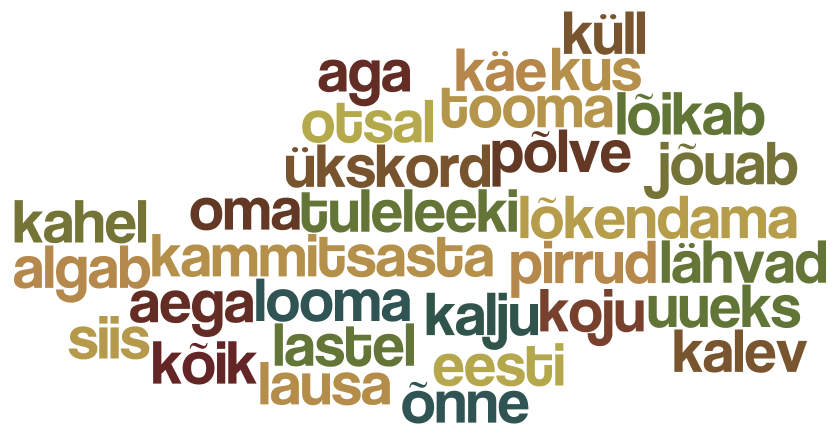
\includegraphics[width=0.9\linewidth]{klpgv}
\caption{Eesti rahvuseepose ,,Kalevipoeg'' viimase kaheksa värsi sõnad}
\allikas{Autori joonis, kasutatud lõiku F. R. Kreutzwaldi teosest
,,Kalevipoeg''}
\label{klpgv}
\end{figure}

Kasutades rohkem mälu saab iga sõna kohta salvestada ka selle esinemiste arvu.
Veel rohkemate ressursside abil saab jälgida sõnapaare või kolmikuid või mingeid
kombinatsioone neist, kuid selliste tunnuste esinemise kohta info kogumiseks on
vaja ka palju rohkem teksti --- erinevaid sõnapaare on palju rohkem kui sõnu.

Selles rakenduses on kasutatud üksikute sõnade esinemiste arvudel põhinevaid
esitusi. Selle otsuse põhjustasid esialgsete mõõtmiste tulemused, mille järgi
sõnapaaride kasutamine tulemust märgatavalt ei parandanud.

\subsection{Dokumendis esinevate sõnade statistiline kirjeldamine}
\label{tfsec}
Termini esinemissagedus (ingl \eng{term frequency}, TF) on intuitiivselt
tõlgendatav kui termini osakaal vaadeldavas tekstis.
Iga sõna TF määrab järgmine avaldis:
\[ tf = \frac{\text{sõna esinemise arv antud tekstis}}{\text{sõnu tekstis
kokku}} \]
\autocite{wiki-term-frequency}
\autocite{peroneTF}

\label{tfidfsec}
IDF (ingl \eng{inverse document frequency}) 
on kokkuleppeline suurus, mis näitab, kui erakordne on termini esimemine suvalises
tekstis, ja kahaneb logaritmiliselt koos terminit sisaldavate tekstide osakaalu
kasvuga.
Tavaliselt kasutatakse järgnevaga sarnast valemit:
\[ idf = -\log \left(\frac{1+\text{tekste, kus esineb see termin}}{\text{tekste kokku}} \right) \] 
%Liidetava \(1\) võib ära jätta, kui kõik vaadeldavad terminid esinevad vähemalt
%ühes vaadeldavas dokumendis --- selle ainus eesmärk on tagada, et funktsiooni
%väärtus oleks alati määratud.
Erinevate dokumentide võimalikult iseloomulikuks eristamiseks kasutatav suurus
TFIDF on lihtsalt kahe kirjeldatu korrutis (\(tfidf = tf \cdot idf \)).
Sel viisil saavutatakse tulemus, kus kus ühe sõna esitamiseks kasutatav arv on
võrdlemisi suur ainult siis, kui sõna on võrdlemisi haruldane (IDF on suur) ja
sõna mitmekordsel esinemisel suureneb seda esinev väärtus veelgi (TF kasvab).
\autocite{wiki-term-frequency}
\autocite{peroneTFIDF}

\chapter{E-kirja struktuur}
Kuigi kasutajale näidatakse e-kirjast vaid loetud välju, on tegelik sõnum palju
mitmekesisem. Siin on kirjeldatud valitud väljade eesmärki ja toimimist.

\section{Sõnumi unikaalne ID}
Sõnumite üksteisest eristamiseks kasutatakse välja \enp{Message-ID}. See peab olema igal
e-kirjal ja selle väärtus ei tohiks kunagi korduda. \enp{Message-ID} peab vormilt olema
terviklik meiliaadress.
Kui sõnum vastab mingile veebiaadressile, võib
unikaalse ID aluseks olla see aadress, muudel juhtudel on soovitatud kasutada
kombinatsiooni kellaajast ja saatja arvuti nimest \autocite{rfc2111}. Vaatamata
nendele nõuetele genereerib näiteks Microsoft Outlook ebakorrektsete
identifitseerimisväljadega sõnumeid. \autocite{wiki-message-id}

\section{Viited eelmistele kirjadele}
Väljad In-Reply-To ja References on teise sõnumi vastuseks saadetud sõnumitele kohustuslikud ja neil
peab olema ära märgitud nende sõnumite Message-ID-d, millele vastati või
viidati.
References väljal peaksid kajastuma ka kõik sõnumid, millele on viidatud
sõnumitest, millele antud sõnum viitab. Sõnumil, mis ei ole vastus ühelegi
teisele sõnumile, ei tohi olla kumbagi neist väljadest. \autocite{rfc5322}

\section{Sõnumi kohaletoimetamise logi}
Väljadel Received hoitakse infot sõnumi teekonna kohta internetis. Täpsemalt lisavad arvutid, mida
sõnum läbib, sinna kirjed selle kohta, milliselt aadressilt ja millal sõnum vastu
võeti. Iga järgmine kirje lisatakse eelmise ette, st viimane kirje on saatjale
kõige lähem \autocite{readheaders}. 
\autocite{rfc5322}
\autocite{rfc5321}

\section{Mitmeosalised sõnumid}
Iga e-kiri võib koosneda mitmest osast, näiteks manused on eraldi osadeks.
Sõnumi osadeks jaotamine ei ole rangelt reguleeritud, kuid iga osa alguses peab
olema Content-Type väli, mis kirjeldab selle osa sisu ja vormi. Osad võivad
omakorda alaosadest koosneda, moodustades puustruktuuri. Üheks sõnumi osaks võib
olla teine terviksõnum, näiteks selle edastamise korral.
\autocite{rfc1521}

\section{Kodeeringud}
Hilisema lisana algsele standardile võib e-kirja põhitekst ja ka enamus
ülejäänud väljadest olla mõnes muus kodeeringus kui 7-bitine ASCII, kuid see
peab olema pakitud 7-bitise ASCII kodeeringu sisse, asendades ASCII kodeeringuga
mitte esitatavad märgid neid ja nende algset kodeeringut kirjeldava
mitmemärgilise kombinatsiooniga või teisendades kogu vastava välja BASE64
süsteemi. \autocite{rfc2047}
\autocite{wiki-unicode-and-email}

Kuigi sidepidamiseks kasutatava kodeeringu kohta määrab RFC 2047 kindlad
reeglid, on selle sisse pakitud teksti kodeering saatja või enamikel juhtudel
tema meilitarkvara valida. Selles töös on tähtis, et juba varem kohatud sõnad,
mille kohta on midagi teada, oleksid ära tuntavad, olenemata konkreetse kirja
kodeeringust, seetõttu tuleb võimaluste piires kõik väljad ühte kodeeringusse
üle viia.

\section{Maildir formaat}
Maildir formaate e-kirjade salvestamiseks loodi algselt qmail meiliserveri
tarbeks, nüüdseks on see \eng{Mbox} formaadi kõrval kujunenud üheks viisiks sõnumite
kindlast rakendusest sõltumatuks salvestamiseks. Seda toetavad meiliklientidest
näiteks Kmail,
Evolution, Mutt, Alpine ja Sup.
\autocite{wiki-maildir}
Kirju on võimalik maildir kataloogi sünkroniseerida POP, IMAP ja veel mitmetest
teistest serveritest, seda näiteks Fetchmail abil \autocite{fetchmail}.

Python programmeerimiskeele standardteegi juurde kuulub moodul \enp{mailbox},
mis lubab hallata maildir, \eng{Mbox} ja teistes vormingutes meilihoidlates olevaid
kirju ja nende metaandmeid \autocite{pymailboxdoc}.

\chapter{Kirjast olulisusega seotud info eraldamine}
Selles peatükis käsitletavate lisatunnuste mõju klassifitseerimisele iseloomustavad
mõõtmised on lisas 10.
\section{Kas konkreetsele kirjale on vastatud?}
Ühelgi standarditega reguleeritaval väljal kirja vastatuse kohta infot ei
salvestata, samuti ei tee seda ka ükski levinum meiliklient omaalgatuslikult
\autocite{KorpelaMailHeaderRef}.
Maildir formaat pakub küll vastuse saanud sõnumite tähistamiseks
lippu ,,R'' \autocite{maildir},
aga hoidmaks sisulist lahendust maildiri kasutamisest või
mittekasutamisest sõltumatuna, ei saa sellele lootma jääda.
Samuti ei märgi lihtsalt maildir formaadi kasutamine vastatud kirju
vastatuks, see on meilikliendi ülesanne ja näiteks antud juhul kirjade
Gmailist salvestamiseks kasutatud programm Offlineimap seda ei teinud.

Universaalsem viis on kasutada ära teiste kirjade In-Rely-To
ja References väljadel leiduvat infot. Kui mingi kirja Message-ID leidub mõne
teise kirja ühel või mõlemal nimetatud väljal, on sellele kirjale vastatud.
Siiski on ka sellel meetodil üks märkimisväärne puudus --- see ei toimi kasutaja
poolt vastatud kirjade jaoks, kui kasutaja saadetud kirju ei ole saadaval.
Selline olukord võib tekkida, kui saadetavaid kirju ei salvestata. Selle
probleemi tagajärgi vähendab asjaolu, et vähemalt kõik meiliprogrammid, millega
autor kokku puutunud on, salvestavad vaikimisi kõik saadetavad kirjad,
vastupidisteks näideteks selgusid veebiotsingu abil ainult üksikud veebipõhiseid
kasutajaliideseid \autocite{yahooSaveSent} \autocite{verioSaveSent}.

\section{Tekst}
Kõige lihtsamast e-kirjast teksti eraldamine on triviaalne, kõik pärast päise
väljadele järgnevat tühja rida ongi tekst. Keerulisemaks teevad olukorra
lisavõimalused, eelkõige mitmeosaliste sõnumite tugi ja erinevate kodeeringute
üksteise sisse pakkimisel põhinev tagasiühilduvus.

Ei saa eeldada, et mitmeosalise sõnumi puhul oleks tekstiosa põhisõnumi otsene
osa, samuti võib see esineda korduvalt erineva sisutüübiga (erinevates kodeeringutes või formaatides, ingl \eng{content type}) või puududa üldse.
Mitme samatüübilise tekstiosa esinemise korral tõlgendab antud uurimuse käigus
valminud programm neid ühe tekstina. Erinevate sisutüüpide korral käsitletakse
ainult ühte - kõige lihtsamat. Manuseid ei avata.
Erinevatest kodeeringutest Unicode kodeeringusse konvertimine on lahendatud,
kasutades kõigepealt ära Pythoni mooduli \enp{mailbox} automaatset
dekodeerimisvõimalust ja vigaste sümbolite esinemise korral need lihtsalt ära
jättes --- tekst mõne(kümne) puuduva tähega on parem kui üldse ilma tekstita.
Samamoodi üritatakse teksti, mille kodeering ei ole otseselt määratud, tõlgendada
nagu see oleks UTF8 Unicode kodeeringus --- UTF8 on võrdlemisi laialt
levinud ja tagasiühilduv veel laiemalt levinult ASCII kodeeringuga, võimalus
sel viisil loetav tekst kätte saada on proovimist väärt.
\autocite{wiki-unicode}

Sarnase loogika alusel on e-kirjast teksti eraldamise teostanud ka
{R. \citeauthor{pyMultilingualMail} \autocite{pyMultilingualMail}}.

\subsection{HTML}
E-kirjas on võimalik lihtteksti asemel sisu edastada ka HTML formaadis,
lubades sellega laia valiku kujundusvõimalusi.
Ideaaljuhul oleks võimalik sel viisil kasutada kõiki veebilehekülgedele omaseid
kujunduselemente, kuid sellega kaasnevate probleemide tõttu ei ole see
üksmeelselt toetatud lahendus. Vaatamata selle vastuolulisele staatusele
saadavad paljud meilikliendid sellise formaadiga sõnumeid vaikevalikuna.
\autocite{wiki-html-email}

Vaadeldud e-kirjade hulgas olnud 999-st HTML osa sisaldanud kirjast vaid 924
pakkusid otseselt alternatiivi (statistika kirjade formaatide kohta on lisas 11).
Ülejäänud 75 oleksid tehnilistel põhjustel
või turvakaalutlustel HTML sisu mitte avavates rakenduses loetamatud. Saamaks
kätte võimalikult palju infot uuritavate kirjade kohta on vajalik kasutada
HTML formaadis sisu.

HTML formaadis sõnumitest teksti eraldamiseks kasutatakse html2text-nimelist
Pythoni moodulit, mis genereerib vaikimisi ASCII teksti, kuid vastavate
seadistustega suudab ka väljastada Unicode teksti
\autocite{html2text}.
Kui samas kirjas on alternatiivselt HTML sõnumile olemas ka lihttekst,
eelistatakse viimast. Muudel juhtudel toimib HTML formaadis teksti käitlemine
nagu lihtteksti puhul, ka teostus on sarnane.

\section{Päise väljade kasutamine}
Tagamaks võimalikult suure arvutile saadaoleva info hulga ja kompenseerimaks
vältimatuid puudujääke, on selles uurimuses kasutatud kirjade klassifitseerimisel
lisaks tekstile ka nende päise väljade sisu. 
Väljade standardijärgne kasutus ja tähendus ei ole antud uurimistöö jaoks oluline,
eesmärk on kaasata kõik väljad, mis võivad põhjendatult kanda infot kirja olulisuse kohta.
Esmajärjekorras peab olema
kirja olulisuse tuvastamisel kättesaadav kogu teave, mida sellest kirjast
kasutajale selle avamisel kuvatakse ja mille järgi kasutajal on võimalik
samalaadne otsus teha. Selle põhimõtte järgi on kaasatud kirja saatjat ja
adressaate näitavad väljad \eng{From}, \eng{To} ja \eng{Cc} ja kirja sisu lühikeseks kirjelduseks
mõeldud väli \eng{Subject}.

Samamoodi analoogiliselt graafilisele kasutajaliidesele,
kus erinevatelt väljadelt pärit tekst paikneb erinevates lahtrites, on kõikidele
päise väljadelt teksti hulka arvatud sõnadele lisatud eesliitena välja nimi.
Erandina on \eng{Subject} välja tekst dubleeritud nii kirja sisu osana, kui eraldi
väljal oleva tekstina --- sõna tähtsus kirja olulisuse suhtes on \eng{Subject} väljal
ja kirja sisus kõikide eelduste kohaselt sarnane.

Väljad \eng{Importance}, \eng{Priority} ja \eng{Precedence}
on vähemalt nime poolest ja ka
praktiliselt seotud kirja tähtsusega. Kuigi kahe esimese kasutuse kõrgaeg
on jäänud ajalukku ja viimane on oma algsest tähendusest kõrvale kaldunud,
ei saa neid lugeda tähtsusetuks \autocite{FalkPrecedence}. Nende väljade täpsem kirjeldus ja ajalugu
väljub aga antud uurimistöö piiridest.
2636 vastavalt uuritud kirjast leidub nimetatud päistest esimest 91 korral (ligikaudu
3,4\%) ja
viimaseid kahte vastavalt seitsmel korral (0,2\%) ja 1489 korral (56,5\%). Kuna on
olemas põhjendatud võimalus, et need sisaldavad infot selle kohta, kas kiri
saab tõenäoliselt vastuse või mitte, on nende sisu kaasatud.

Veel on kaasatud väljad \eng{List-Id} ja \eng{X-Mailer}, mis vastavalt kirjeldavad
postloendit, mille kaudu kiri saadeti, ja selleks kasutatud programmi. Kuigi
puudub otsene seos kirja tähtsusega ja enamus autori kasutatud meilikliente
nende sisu kasutajale ei avalda, on need kaasatud kirjade klassifitseerimisel,
eraldi esindamaks erinevatest postiloenditest ja keskkondadest pärit kirjade
tähtsust.

\section{Saatja soo hindamine}
Lisaks iga saatja eraldi käsitlemisele läbi tema aadressi esinemise \eng{From} väljal
peetakse üldistavalt arvet ka erinevast soost saatjate üle. Kuigi selline
üldistus võib tunduda liigne, on see üllatavalt informatiivne. Kasutatud kirjade
järgi on tõenäosus, et kiri, mille kohta on ainult teada, et see tuli naissoost
isikult, saab vastuse üle kolme korra suurem, kui samasugune kiri mehelt.

Saatja sugu määratakse \eng{From} väljal oleva nime järgi, kasutades vastavat tasuta
veebiteenust firmalt Rapidleaf \autocite{RapidLeafGender}
 ja salvestades nimed, mille sugu on juba teada, korduvate päringute vältimiseks.

Kuigi uurimistöö valmimise ajal avas sama firma ka teenuse fraasist
nime eraldamiseks, eraldab valminud rakendus nime \eng{From} realt ise. Selline
lähenemine saadab võõrale firmale vähem infot kasutaja isiklike kirjade kohta
ja jätab nime tuvastamise viisi asendatavaks --- kui kõnealune veebiteenus
peaks toimimise lõpetama on võimalik minna üle näiteks rahvaloenduse tulemuste
kasutamisele.

\section{Saatja asukoha hindamine}
Analoogselt saatja soole on võimalik üldistada ka kirja umbkaudse
saatmiskoha alusel. Selle leidmiseks on antud uurimistöö käigus valminud
programmis kasutatud viimasel Received väljal oleva päritoluaadressi asukoha
leidmist GeoIP andmebaasist, mille tasuta versioon määratleb vastuse riigi
täpsusega. \autocite{MaxmindGeoIP}

Ootuspäraselt on sellise üldistuse juures uuritud postkastis olnud kirjade järgi
tõenäosus, et vastatakse kasutaja kodumaalt (Eestist) pärit kirjale ,suurem kui
tõenäosus, et vastatakse näiteks Ameerika Ühendriikidest pärit kirjale, antud
juhul oli erinevust ligikaudu 1,4 korda.

\section{E-kirja keel}
Veel üks potentsiaalselt informatiivne väga üldistav tunnus kirja olulisuse
kohta on selle keel. Keele tuvastamiseks on kasutatud omakorda statistikat,
täpsemini kolmetäheliste tähekombinatsioonide sageduse ja kodeeringu järgi
keele tuvastamist mooduli \enp{language-guess} abil
\autocite{GuessLanguegePYPI}.

Keele tuvastamine on siin kirjeldatud tunnuste hankimistest kõige
arvutuslikult mahukam operatsioon. 

Tõenäosus, et suvaline eestikeelne kiri vaadeldud kirjade hulgast saab vastuse,
on 25 korda suurem kui inglisekeelse kirja puhul.

\chapter{Erinevate lahenduste võrdlus}
\section{Masinõppealgoritmide implementatsiooni valik}
Kõikide selle uurimuse raames tehtud mõõtmiste juures on kasutatud scikit-learn
implementatsioone vajalikest algoritmidest, mille uuesti programmeerimine oleks
tulutu ja aeganõudev. Sellise valiku põhjuseks on asjaolu, et scikit-learn
ühildub programmeerimiskeelega Python, milles kirjutatud programm on madalama
astme keeltega võrreldes suhteliselt
kergesti loetav \autocite{wiki-python-programming-language}. Samuti oli Pythoni
kasutamise taga asjaolu, et just sellega on seotud suur osa autori eelnevast
programmeerimiskogemusest.

\section{Kasutatud e-kirjad}
Kogu uurimis- ja arendustegevuse käigus kasutati ainult autori isiklikku
kirjakasti keskkonnast Gmail. Reaalkooli postkastis asuvad kirjad jäid
tehniliste probleemide tõttu kasutamata, kuid nende puudumine ei mõjuta
tulemuse tõepärasust: kirjade sisu moodustab niigi ainult murdosa lugejale
nende tähtsuse üle otsustamisel saada olevast infost, väikse osa kirjade
eemaldamine olukorda ei muuda. Mõlemal juhul, peab rakendus hakkama saama
valikulise, piiratud informatsiooniga.

Teiste inimeste kirjade kaasamist
kaaluti, aga selle puudused kaalusid üles lisaandmetest saadava tulemuse.
Võõraste kirjade käitlemine vajab kahepoolset usaldust, sellega kaasnevad
vastutus ja piirangud, mis oleksid olulisel määral vähendanud selle
kasulikkust. Esiteks, ei ole lihtne leida inimest, kes kogu oma isikliku
kirjavahetuse ka hea eesmärgi nimel kellelegi uurida annaks. Kahjuks
ka nõusoleku olemasolul ei õnnestunud pereliikmete meile tehnilistel
põhjustel terviklikul kujul salvestada. Konfidentsiaalsete kirjade välja
jätmine oleks tähendanud katsealuste kirjade omanikule suurt lisatööd ja
sellega saadud tulemus ei pruugi enam olla samaväärne terve postkastiga
töötamisega.

Kokku oli kasutusel 2942 kirja, millest 336 olid saadetud ja 2606
vastuvõetud kirjad. Saadetud kirju kasutatud ainult vastuvõetud kirjade vastuse saamise järgi kaheks jaotamiseks.
Vastuvõetud kirjadest 91 olid saanud vastavalt märgistatud e-kirja kujul vastuse ja loeti seetõttu oluliseks.

\section{Mõõtmisprogramm}
Tulemuste võrdlemiseks vajalike graafikute koostamiseks loodi valminud rakenduse
algvariant nii, et see suudaks etteantud klassifitseerimisviiside kohta
ROC kõvera ja \eng{precision} ja \eng{recall} vahelise seose graafiku koostada.
Sellise otsuse põhjuseks oli eekõige mainitud protsessi jaoks vajalike arvutuste
suur hulk, samuti vajadus seda näiteks kasutatavate tunnuste muutmise järel
korrata ja uut tulemust eelmisega võrrelda.

Vältimaks mõõtmistulemuste märkimisväärset erinemist praktikas saavutatavast
oluliste kirjade tuvastamise kvaliteedist mõõdeti iga klassifitseerimisviisi
andmed kümme (esialgsetel mõõtmistel viis) korda, luues iga kord enamike kirjade abil mudel,
millega klassifitseeriti ülejäänud kümnendik (või viiendik) kirju. Iga selline alammõõtmine
kanti ka graafikule, mis on saadaval lisades.

Mõõtmise alguses viiakse kõik kirjad teksti kujule, esitades kõik võimalikud
tunnused. Tegu on protsessi kõige aeganõudvama osaga ja selle kordamine ei
oleks otstarbekas. \label{howmeasure}
Kirjad jagatakse scikit-learn funktsiooni \enp{StratifiedKFold} abil kümnesse
gruppi nii, et igas grupis on vastuse saanud kirjade osakaal ligikaudu sama.
Iga grupiga läbitakse järgmine protseduur:
\begin{itemize}
    \item Vaadeldava grupi kirjad (testandmed) eraldatakse ülejäänud kirjadest (treeningandmed),
        mille abil luuakse mudel esimeste klassifitseerimiseks.
    \item Mõlemale grupile rakendatakse vektorkujule viimise eelne teisendus,
        näiteks eemaldatakse kirja keelt esitav tunnus, mille puudumise mõju soovitakse hinnata.
    \item Testandmed viiakse üle vektorkujule.
    \item Treeningandmed viiakse üle testandmetega sama struktuuriga vektorkujule.
    \item Testandmetele ja treeningandmetele rakendatakse järgmine teisendus,
        näiteks minnakse üle sõnade esinemiste arvudelt TF esitusele.
    \item Luuakse treeningandmete abil mudel.
    \item Ennustatakse loodud mudeli põhjal iga testandmete hulka kuuluvad
        kirja kohta, kas see on saanud vastuse.
    \item Salvestatakse mõõtmise tulemus listi, millest see hiljem graafikule kantakse.
\end{itemize}

Pärast antud käivitusel määratud mõõtmiste tegemist salvestas programm kõik
valminud graafikud etteantud nimedega uude kuupäeva ja kellaaja järgi nimetatud
kausta ja kopeeris sinna ka koopia iseenda koodist. Viimase puhul oli tegemist
kontrollmeetmega --- kui hiljem tekib vajadus mõne mõõtmistulemuse
tagamaid lähemalt uurida, on kogu info selle jaoks olemas.

\section{Jooniste tõlgendamine}
Põhiliselt kasutati erinevate meetodite võrdlemiseks ROC ja \eng{precision-recall}
graafikuid. Muude piirkondadega võrreldes eriti tähtis on graafiku osa, mis
näitab klassifitseerimise edukust olukorras, kus tuleb eelkõige võimalikult
paljud olulised sõnumid ära tunda ja ebaoluliste sõnumite mitte valesti
oluliseks lugemine on selle kõrval teisejärguline. Sellisele kasutusele sobivaks
kujunes parimate lahenduste juures 90\% tähtsatest kirjadest õigesti ära tundev lävend,
millele vastas valetuvastuste hulk 15\% mitteolulistest kirjadest.

Kirjeldatud andmete põhjal on selles töös e-kirjade vastuse saamise või
mittesaamise ennustamiseks kasutatud kolme erinevat viisi kirja üksikute
tunnuste põhjal arvude jadana esitada --- \eng{Counts}, TF ja TFIDF ---
ja nende jadade vastavaks klassifitseerimiseks on kasutatud kolme meetodit:
SVC lineaarse tuumaga (joonistel linearSVC), SVC RBF \eng{radial
basis function} tuumaga (joonistel rbfSVC) ja
multinomiaalne naiivne Bayesi klassifitseerija (joonistel MNB).

Enamik joonistest
kajastavad kümne või viie üksteist kontrolliva katse keskmist tulemust. Üksikut katset kirjeldavatel joonistel on jooned poole võrra kitsamad ja legendil on sõna \eng{fold}.

\begin{figure}[ht]
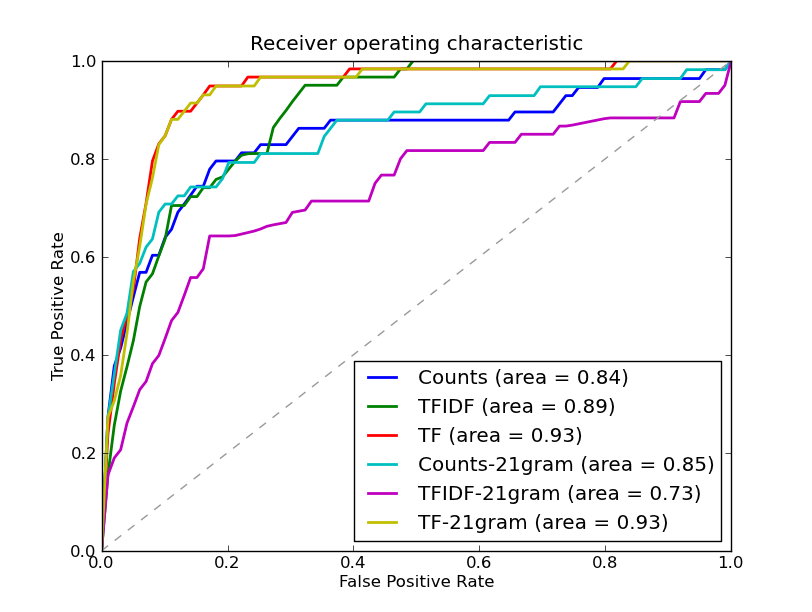
\includegraphics[width=\linewidth]{1+21grams}
\caption{Erinevate teksti numbrilise esitamise meetodite võrdlus}
 % \allikas{Autori joonis}
\label{textvect21}
\end{figure}

\section{Teksti esitamise meetodite võrdlus}
Joonisel \ref{textvect21} on kuue erineva teksti esitamise viisiga saavutatav ROC-kõver lineaarse SVM klassifitseerija kasutamisel.
Kõikidel katsetel on kasutatud lineaarset SVM klassifitseerijat.
\eng{Counts} tähistab esitusviisi, kus iga kirja kohta on tähistatud, mitu korda iga
sõna selles esineb, TF ja TFIDF on selle juba kirjeldatud teisendused.
Katsed, kus lisaks üksikutele sõnadele jälgiti ka sõnapaare, on tähisega 21gram.
Nagu ka kõikidel järgnevatel graafikutel on joone tähise taha märgitud selle
alune pindala. ROC kõveratel esinev hall diagonaaljoon tähistab hüpoteetilise
suvaliselt kirju klassifitseeriva algoritmi tulemust ja on välja toodud
võrdlemise lihtsustamiseks.

Võrreldes \eng{Counts} ning \eng{Counts}-21gram kõveraid, võib näha, et erinevust praktiliselt
ei ole, sama kehtib TF ning TF-21gram kõverate kohta. TFIDF ning TFIDF-21gram
kõveraid võrreldes aga selgub, et katses, kus jälgiti sõnapaare, oli enamike
valesti oluliseks loetavate kirjade osakaalude juures õigesti oluliseks loetud kirjade osakaal palju väiksem kui katses,
kus sõnapaare kasutatud. See tähendab, et kui mingi kindel protsent kirjadest,
mis tegelikult olulised ei olnud, selleks loeti, siis samal ajal tundis programm 
sõnapaare kasutava katse puhul ära väiksema osa kirjadest, mis tegelikult 
olulised olid, kui sõnapaare mitte kasutav katse. Seega sõnapaaride kasutamine 
kasu ei toonud, halvemal juhul oli mõju isegi selgelt negatiivne

Esimese tähelepaneku põhjus seisneb saadaoleva teksti
vähesuses: enamik sõnapaarid esinevad vaid ühe korra ja seetõttu nende abil
uue kirja kohta mingeid järeldusi teha ei saa, kuna need
ei oma esimesel kohtamisel mingit infot kirja olulisuse kohta.
TFIDF kaotab sama probleemi tõttu efektiivsust ka sõnapaare ignoreeriva
lahendusega võrreldes, kuna ainult ühes dokumendis esineva sõnapaari IDF väärtus
ja seetõttu ka kaal otsustamisel on palju suurem, kui korduvalt esineva sõna
oma.
Sarnased tendentsid väljenduvad ka lisas 1 \todo{LISAnumber}
paikneval ainult sõnapaaride kasutamist üksikute sõnade kasutamisega võrdleval
graafikul.

\begin{table}[h!]
\caption{Edaspidi mudelite loomisel kasutatud parameetrid}
\label{paramtabel}
\begin{tabular}{| l | l | l |} \hline
klassifitseerija & mõõtmised & valitud väärtused \\ \hline
lineaarne tugivektorklassifitseerija &
    lisas 7 &
    \( C = 2 \) \\ \hline
RBF tuumaga tugivektorklassifitseerija &
    lisas 8 &
    \( C = 4;\; \gamma = 1\) \\ \hline
multinomiaalse naiivne Bayesi klassifitseerija &
    lisas 9 &
    \( \alpha = 10^{-3} \) \\ \hline
\end{tabular}
\end{table}


\section{Matemaatiliste mudelite parameetrite valimine}
Kõikidel siin vaadeldud klassifitseerimismudelitel on parameetrid, mille
abil saab nende toimimist mõjutada. Selliste väärtuste valimisel sai lähtutud
eesmärgist saada katseliselt kirjad võimalikult hästi klassifitseeritud.
Erinevate parameetrite või nende kombinatsioonide headust hinnati ROC ja
precision-recall kõverate võrdlemise teel. Vajadusel määrati ühe
katsega parameetri ligikaudne väärtus ja seda täpsustati teise katsega.
Kuigi sellisel viisil tulemus ei ole absoluutselt täpne, on see aktsepteeritav,
kuna erinevate kirjakomplektide puhul on ideaalsed parameetrite väärtused
väiksel määral erinevad, tähtis on aga üldiselt hea tulemuse saavutamine.
Ülevaade valitud parameetritest on tabelis \ref{paramtabel}.


\section{Võimalike lahenduste võrdlus}
\begin{figure}
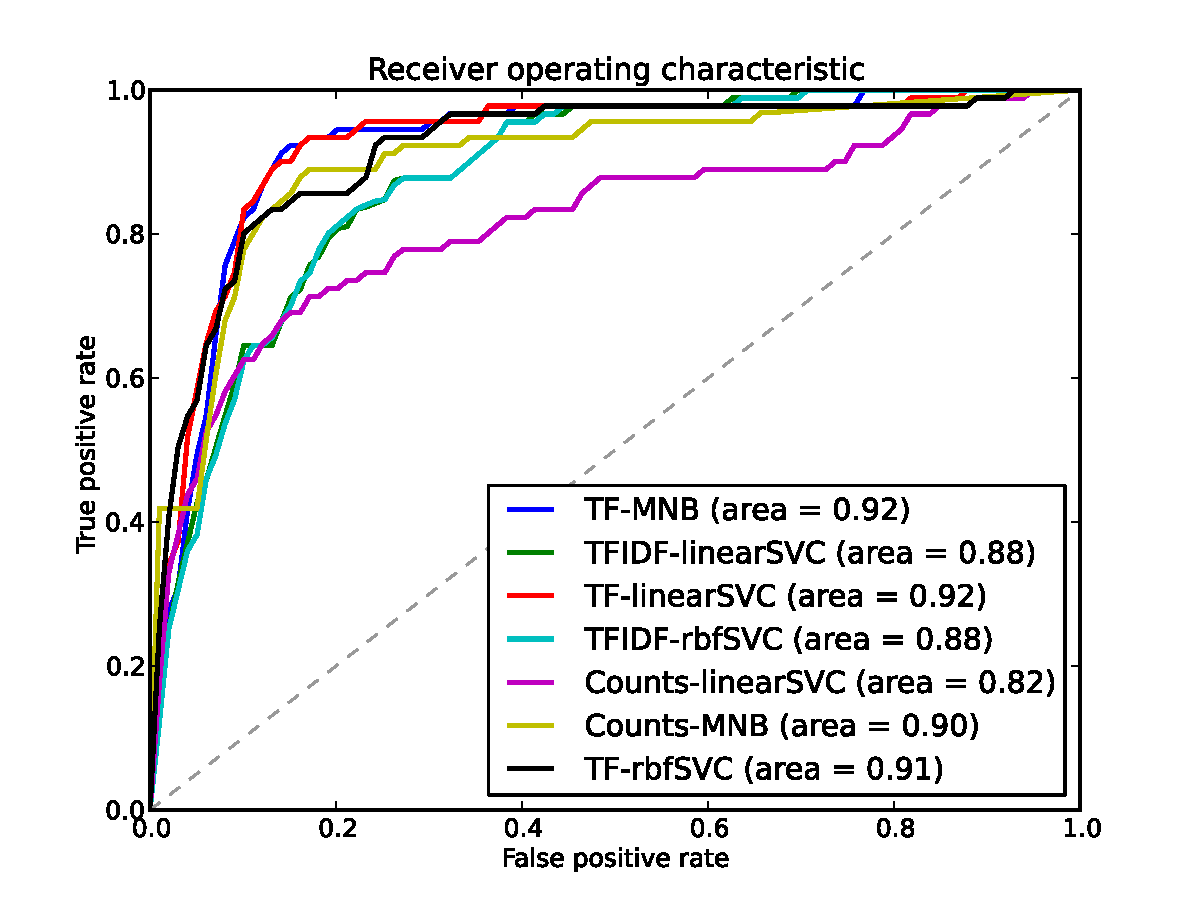
\includegraphics[width=0.93\linewidth]{finalroc}
\caption{Erinevate klassifitseerijate ja teisenduste suhteliste töökarekteristikute kõverad}
 % \allikas{Autori joonis}
\label{finalroc}
\end{figure}

\begin{figure}
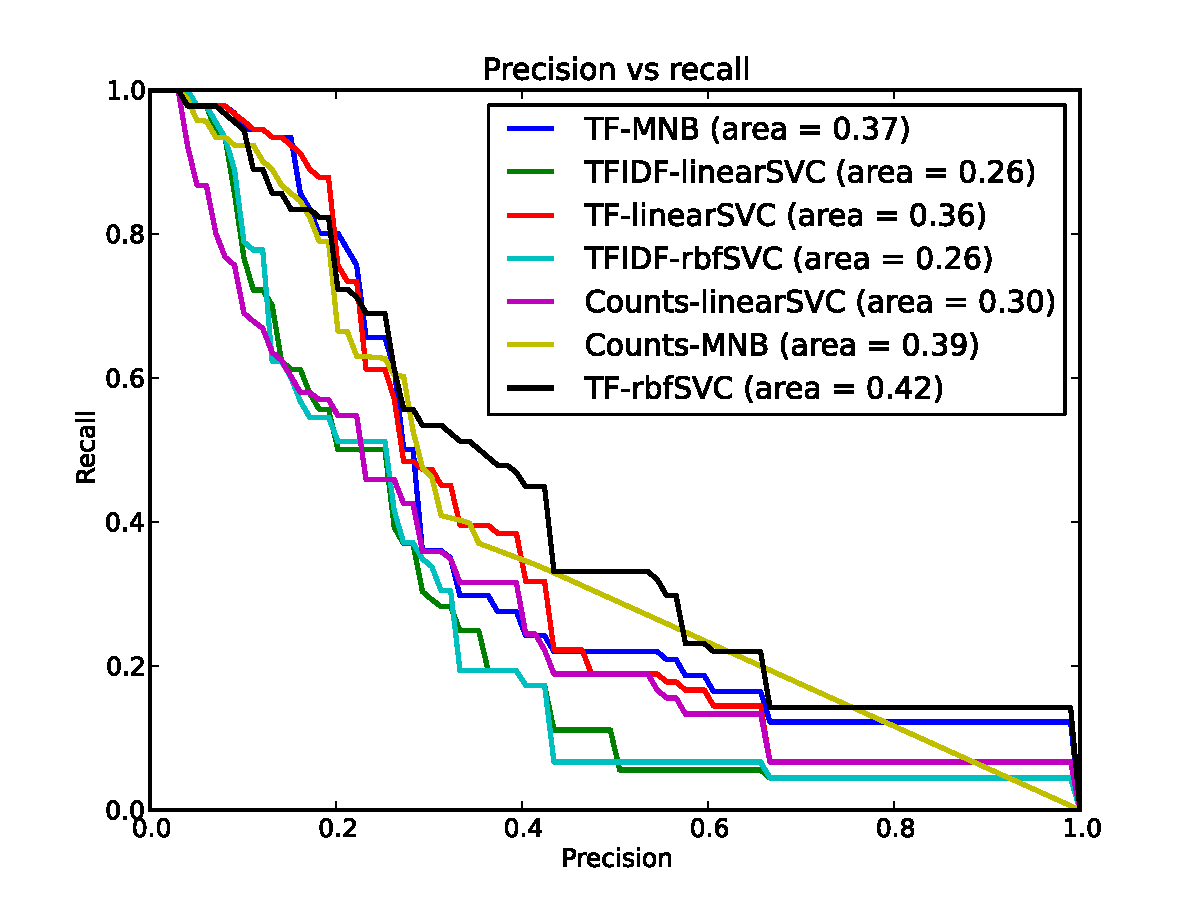
\includegraphics[width=0.93\linewidth]{finalprrec}
\caption{Erinevate klassifitseerijate ja teisenduste \eng{precision} ja \eng{recall} vaheline seos}
 % \allikas{Autori joonis}
\label{finalprrec}
\end{figure}

Selles alapeatükis võrreldakse omavahel kirjeldatud viise kirjade klassifitseerimiseks.
9 vaadeldavat lahendust on kombinatsioonid kolmest
klassifitseerijast ja kolmest sisendvektori teisendusest.
Kuna teisendused avaldavad klassifitseerijatele erinevat mõju, siis tuleb
nende osas valik teha korraga. Kõigi variantide ROC kõverad on joonisel \ref{finalroc}
ja \emph{precision} ja \emph{recall} vahelised seosed joonisel \ref{finalprrec}.
Üksikute katsete graafikud ja siin esitatud graafikute vektorgraafikaversioonid on saadaval lisas 2\todo{LISAnumber}.

Teistest märgatavalt halvemini saavad ülesandega hakkama töötlemata tunnuste
esinemise arve kasutav RBF tuumaga tugivektorklassifitseerija ja TFIDF
vektoritega opereeriv multinomiaalne naiivne Bayesi klassifitseerija, kusjuures
esimene suutis väikse hulga vastatud kirju ülejäänute hulgast ära tunda ainult ühel katsel kümnest
ja viimane ei suuda ühtegi kirja vastatuks lugeda.
Kuna selliste tulemuste graafikul kujutamine neid täpsemini ei iseloomustaks,
on need selguse huvides põhiosa joonistelt eemaldatud (saadaval lisas 3\todo{LISAnumber}).

Multinomiaalse Bayesi klassifitseerija puhul tasub tähele panna, et kuigi
selle kasutamisel TFIDF teisendusega oli tulemus halvim võimalik, siis
ainult TF rakendamisel töötas sama meetod ühena parimatest. Erinevuste põhjusteks
on konkreetse scikit-learn teegi teostuse omadus käidelda korrektselt vaid
täisarve, muudel juhtumitel ei ole õige tulemus garanteeritud \autocite{sklearnMNB}.
Erinevuse TF ja TFIDF kasutamisel saadud tulemuste vahel põhjustas see,
et kuigi mõlema katse puhul analüüsis multinomiaalne Bayesi klassifitseerija
ujukomaarve, siis TF korral kasutati vaid ühe jagamise teel saadud arve,
%(konkreetsete tunnuste esinemise arvu ning kõigi kirjas olevate tunnuste arvude
%jagatis, täpsemalt on protsessi kirjeldatud leheküljel \pageref{tfsec})
TFIDF kasutamise korral oli sama jagatis läbi korrutatud ka teise 
jagatise logaritmiga,
% (IDF, täpsemalt vt leheküljelt \pageref{tfidfsec})
mille vältimatu ebatäpsuse tõttu tekkisid vead.

Iga tugivektorklassifitseerija kasutamine töötlemata tunnuste esinemiste arvude
vektoritega jääb eeltöötlemisega variantidele alla. Selle põhjuseks taga on
asjaolu, et SVM algoritm põhineb sisendi geomeetrilisel interpretatsioonil,
mis tahtmatult ja kontrollimatult omistab tähtsust näiteks kirja pikkusele.
TF ja IDF vähendavad otseselt sõnumite erineva pikkuse mõju klassifitseerija
otsusele --- kõikide tunnuste väärtused jagatakse sellega läbi, minnes seeläbi
üle tunnuste suhtelise tähtsuse jälgimisele.

Üllatavalt hästi sai ülesandega hakkama vaid töötlemata tunnuste esinemise arve
kasutav multinomiaalne Bayesi klassifitseerija. Sisulise poole pealt on tegemist
ühe kõige lihtsama käesolevas uurimistöös käsitletud klassifitseerimismeetodiga,
tulemus aga ei jää märkimisväärselt alla parimatele lahendustele ja on kohati
isegi parem palju keerulisematest tugivektorklassifitseerijatest.

TF teisenduse läbinud sisendiga saavutas multinomiaalse Bayesi klassifitseerijaga
sarnase tulemuse ka lineaarne tugivektorklassifitseerija, tuvastades õigesti
vastatuks 85\% meili teel vastuse saanud kirjadest ja lugedes vastatuks veel 10\%
kirju, millele vastuse saamise kohta märget ei olnud. Nende kahe klassifitseerija
tulemused kattuvad peaaegu täpselt ning viitavad üldjoontes heale tuvastavusele,
kinnitades seeläbi hüpoteesi, et kirja sisu abil on võimalik olemasolevate
meetoditega selle olulisust automaatselt tuvastada. Veelgi enam, fakt,
et kaks täiesti erineva tööpõhimõttega meetodit saavad väga sarnase tulemuse,
näitab, et tuvastamine on üldistuv.


\section{Näidisrakendus}
Kuna saavutatud tulemused oluliste kirjade tuvastamisel olid paljulubavad,
sai loodud rakendus arvutisse salvestatud kirjade samal meetodil
klassifitseerimiseks. Järgnev kirjeldab selle toimimist ja erinevusi mõõtmisprogrammist,
näide kasutamisest on joonisel \ref{exampleout}, väljund kajastab kahte olulist ja ühte ebaolulist kirja.
Rakenduse täielik kood on lisas 4\todo{LISAnumber}.

\subsection{Sisend ja väljund}
Rakendus on kasutatav käsurealt. Argumentideks tuleb anda meilide asukoht,
loodava või kasutatava mudeli asukoht ja e-kirjade omaniku meiliaadress.
Neljandaks ja mittekohustuslikuks argumendiks
võib lisada sõna \enp{train}, mille korral luuakse etteantud kirjade abil
uus mudel, mida hiljem saab (ilma seda argumenti lisamata käivitades) kasutada
teiste kirjade klassifitseerimiseks.

Meilide asukohaks võib olla \enp{Maildir} kataloogipuu, või tavaline kataloog,
milles on meilid salvestatud RFC822 standardile vastaval kujul, milles neid ka üle võrgu
saadetakse või \enp{Maildir} kataloogis hoitakse.
Samuti kehtivad Unixi-stiilis metamärgid nagu \texttt{*} ja \texttt{?}.

Väljundiks on mudeli loomise korral mudel ise, mis salvestatakse teise argumendiga määratud.
Uute kirjade kohta ennustuse tegemisel kirjutatakse standardväljundisse iga
kirja kohta üks rida, millel on püstkriipsudega eraldatult saatja aadress,
teema ja hinnang selle kirja olulisusele arvuna lõigust \( [0;1] \). Suur arv
tähistab hinnanguliselt tähtsat sõnumit, väga väike arv vähetähtsat.
Väga väikeste arvude väljastamise kasutatakse koma järel olevate nullide
välja kirjutamise asemel eksponentkuju, kus \texttt{2e-12} tähistab arvu \( 2 \cdot 10^{-12} \).
Info kirjade kohta väljastatakse hinnangulise tähtsuse järjekorras, kus
olulisemad kirjad on eespool.

\begin{figure}[h!]
\vspace{3mm}
\begin{verbatim}
andres@ar:~$ ./olulisedkirjad.py ./mail/cur/ ./model.pc andres.erbsen train
Maildir read.
training
andres@ar:~$ ./olulisedkirjad.py ./mail/new/ ./model.pc andres.erbsen
predicting
kt@ut.ee            | Re: Oluliste kirjade tuvastamine masinppega | 0.87
inga@tlu.ee         | Re: Informaatika olmpiaad 2010 õppimine     | 0.81
noreply@lockerz.com | Kalev Karp has invited you          | 2.56e-09
\end{verbatim}
\vspace{-3mm}
\caption{Näidisrakenduse väljund.}
\label{exampleout}
\end{figure}

\subsection{Klassifitseerimine}
Kuna erinevate klassifitseerimisviiside võrdlemisel saavutati mitme erineva
meetodiga ligikaudu samaväärne tulemus, sai näidisrakenduses kasutatava
klassifitseerija valimisel otsustavaks lihtsuse põhimõtte --- lihtsama
matemaatilise tööpõhimõtte ja teostusega algoritm võib olla teistest töökindlam
ja kindlasti on seda kõige lihtsam kontrollida. Selleks oli häid tulemusi
andnud meetodite hulgast multinomiaalne naiivne Bayesi klassifitseerija (MNB), mille
lihtsama variandi tööpõhimõte on ka selles uurimistöös ära toodud. Teksti
vektorina esitamiseks kasutatakse TF, kuna just sellega andis MNB häid tulemusi.

Väljundisse jõudvad arvud on MNB hinnangud tõenäosusele, et vaadeldav kiri
saab vastuse.

\subsection{Kiirus}
Kasutaja jaoks on oluline ka kirjade tuvastamise kiirus. Kuna programmile ei
anta töötamiseks aega igavesti, siis on tarvis, et töötsükkel oleks võimalikult
optimaalne. Väikesed jäereleandmised kvaliteedis on tööaja lühendamise nimel
õigustatud.

Kirja keele eraldi tuvastamine \enp{language-guess} abil on aeglane. 49 kirja
klassifitseerimisest koosnenud testi läbimiseks kulus seda kasutaval lahendusel
24,7 sekundit, kusjuures keelt mitte tuvastav lahendus sai sama ülesandega hakkama
1,4 sekundiga. Täpne info kogu näidisrakenduse ajakasutuse kohta on saadaval lisas 5\todo{LISAnumber}. 
18-kordne võit kiiruses on väärtuslik, eriti kui kvaliteet oluliselt ei lange.
Lisast \todo{LISAnumber} on näha, et otsese keeleinfo puudumine TF-MNB kombinatsiooni
tööd märkimisväärselt ei sega --- erinevus jääb alla 1\%.

Ilma keeletuvastuseta moodustab põhilise osa programmi tööajast (vt lisa 6\todo{LISAnumber}) Pythoni
dünaamilisele keelele omane lisatöö ja ebaefektiivse standardse andmetüübi
kasutamine teksti hoidmiseks. Samuti oleks võimalik saavutada võitu ajas ja mälukasutused
lugedes e-kirju failist mällu osaliselt ja ainult vajaduse korral.
Kuna selle uurimistöö eesmärgiks ei olnud luua võimalikult kiiret rakendust
jäetakse need täiendused praegu tegemata, kuna nii keelevahetus kui andmehalduse
optimeerimine vähendaksid oluliselt programmi koodi loetavust ja näitlikkust.
Samuti peaks olema lahendus, mis suudab sülearvutil klassifitseerida paarkümmend
kirja sekundis, kodukasutaja jaoks piisavalt kiire.

\subsection{Nõudmised süsteemile}
Rakenduse täieliku funktsionaalsuse kasutamiseks on vajalik järgmiste teekide või nende funktsionaalst pakkuvate 
vastavate alternatiivide olemasolu:
\begin{itemize}
    \item Python 2.7
    \item scikit-learn 0.10
    \item html2text HTML kirjadest teksti eraldamiseks
    \item GeoIP Python API saatja asukoha hindamiseks
    \item language-guess kirja keele tuvastamiseks
\end{itemize}
Arendus toimus Ubuntu operatsioonisüsteemiga arvutis, testimiseks kasutati
ka Arch Linuxit.

\addchap{Kokkuvõte}

Hüpotees, et konkreetse e-kirja ja eelmiste kirjade sisu järgi on arvutil võimalik
olemasolevaid masinõppealgoritme kasutades anda kasulik hinnang kirja olulisusele,
leidis kinnitust. Nii multinomiaalne naiivne Bayesi klassifitseerija kui ka
tugivektorklassifitseerija suutsid 2606 vastuvõetud kirja hulgast
ära tunda 90\% kirjadest, mis olid saanud vastuse, lugedes seejuures oluliseks
veel 15\% kirjadest, mis ei olnud saanud vastavalt märgistatud meili kujul vastust.
Mõlemad parima tulemuse saavutanud lahendused kasutasid TF vektoreid kirjas
leiduvate tunnuste esitamiseks.

Vaid napilt jäid parimatele lahendustele alla TF sisendvektoreid kasutav
RBF tuumaga tugivektorklassifitseerija ja tunnuste esinemiste arve kasutav
multinomiaalne Bayesi klassifitseerija, mõlemad suutsid vaadeldud kirjakomplektis
15\% valetuvastuste hinnaga juures ära tunda 85\% vastuse saanud kirjadest.

Tõhususelt kolmanda grupi moodustasid TFIDF sisendvektoreid kasutavad
tugivektorklassifitseerijad lineaarse ja RBF tuumaga ja tunnuste esinemiste arve kasutav lineaarne tugivektorklassifitseerija, tuvastades sama
valetuvastuste hulga juures õigesti oluliseks ainult 65\% vastuse saanud kirjadest.
Viimast kirjeldatut eristab eelmisest kahest kehvem tulemus 20\% valetuvastuste korral,
kus see luges oluliseks 70\% vastatud kirjadest, eelmised kaks aga 80\%.

Antud ülesande jaoks osutusid sobimatuks RBF tuumaga tugivektorklassifitseerija
kasutamine tunnuste arvudega ja multinomiaalne naiivne Bayesi klassifitseerija
TFIDF sisendvektoritega.

Uurimistöö tulemuste demonstreerimiseks ja esmaseks rakendamiseks loodi programm,
mis suudab \eng{Maildir} formaadis kirjade järgi luua mudeli konkreetse kasutaja
jaoks kirja olulisust näitavate tunnuste kohta ja selle mudeli abil (uute)
kirjade tähtsust hinnata ja neid selle järgi järjestada.

Käesolevas uurimistöös loeti oluliseks kirjad, mis olid saanud vastavalt
märgistatud e-kirja kujul vastuse. Sellise otsuse põhjustas tulemuse
konkreetsus ja üheseltmõistetavus ning autori hinnangul mõistlik eeldus,
et suur osa vastuse saanud kirjadest
on olulised. Sellisel juhul saaks sarnasuse alusel ära tunda ka
olulised, kuid vastust mitte saavad kirjad.
Selle eelduse kontrollimine jääb pigem sotsiaalteaduse valdkonda.


\printbibliography

\addchap{Lisade nimekiri}
Kõik lisad on paberikulu vähendamiseks ja täpsema esituse tagamiseks digitaalkandjal.
\begin{enumerate}
\item Sõnapaaride kasutamine tunnustena (mõõtmistulemused)
\item Seitsme võrreldud lahenduse üksikasjalikud tulemused
\item Kahe kirjade klassifitseerimiseks sobimatu lahenduse tulemused
\item Näidisrakendus kirjade klassifitseerimiseks
\item Näidisrakenduse ajakulu profiilid koos ja ilma keeletuvastuseta
\item Keeletuvastuse mõju klassifitseerimistulemusele
\item Lineaarsve tugivektorklassifitseerija tulemused erinevate parameetri C väärtustega
\item RBF kerneliga tugivektorklassifitseerija tulemused erinevate parameetrit C ja \(\gamma\) väärtustega
\item Multinomiaalse naiivse Bayesi klassifitseerija tulemused erinevate parameetri \(\alpha\) väärtustega
\item Lisatunnuste kasutamise mõju klassifitseerimistulemusele
\item Vaadeldud kirjades esinenud sisutüübid
\end{enumerate}
% to pedantically follow the school rules:
%\addcontentsline{toc}{chapter}{Lisa 1 Sõnapaaride kasutamine tunnustena (mõõtmistulemused)}
%\addcontentsline{toc}{chapter}{Lisa 2 Seitsme võrreldud lahenduse üksikasjalikud tulemused}
%\addcontentsline{toc}{chapter}{Lisa 3 Kahe kirjade klassifitseerimiseks sobimatu lahenduse tulemused}
%\addcontentsline{toc}{chapter}{Lisa 4 Näidisrakendus kirjade klassifitseerimiseks}
%\addcontentsline{toc}{chapter}{Lisa 5 Näidisrakenduse ajakulu profiilid koos ja ilma keeletuvastuseta}
%\addcontentsline{toc}{chapter}{Lisa 6 Keeletuvastuse mõju klassifitseerimistulemusele}
%\addcontentsline{toc}{chapter}{Lisa 7 Lineaarsve tugivektorklassifitseerija tulemused erinevate parameetri C väärtustega}
%\addcontentsline{toc}{chapter}{Lisa 8 RBF kerneliga tugivektorklassifitseerija tulemused erinevate parameetrit C ja \(\gamma\) väärtustega}
%\addcontentsline{toc}{chapter}{Lisa 9 Multinomiaalse naiivse Bayesi klassifitseerija tulemused erinevate parameetri \(\alpha\) väärtustega}
%\addcontentsline{toc}{chapter}{Lisa 10 Lisatunnuste kasutamise mõju klassifitseerimistulemusele}
%\addcontentsline{toc}{chapter}{Lisa 11 Vaadeldud kirjades esinenud sisutüübid}

% \kinnitusleht

\addchap{Resümee}
E-post on üks kõige laiemalt levinud internetikommunikatsiooni
vahenditest. Saabuvate kirjade ülevaatamine ja sellele reageerimine on aeganõudev.
Olukorda parandaks võimalus vaadata kiiresti läbi ainult olulisemad kirjad.

Käesolev uurimistöö käsitleb kindlale isikule oluliste e-kirjade
automaatset ja sõltumatut
äratundmist talle saabuvate kirjade hulgast
ilma kasutaja aktiivse abita.
Oluliseks loetakse vastuse saanud kirju.

Iga kiri esitatakse tunnuste esinemiste arvude, TF või TFIDF vektorina,
kasutades tunnustena kirjas ja selle päise väljadel saada olevat infot.
Selliste vektorite klassifitseerimiseks rakendatakse lineaarse ja RBF
kerneliga tugivektorklassifitseerijaid (SVC) ja multinomiaalset naiivset
Bayesi (MNB) klassifitseerijat. Erinevaid lahendusi on võrreldud ja koostatud
näidisrakendus kirjade klassifitseerimise demonstreerimiseks.

Saavutatud tulemuste kohta on mõõdetud \eng{precision} ja \eng{recall} ning
koostatud suhteliste töökarakteristikute kõverad (ROC).
Hüpotees, et konkreetse e-kirja ja eelmiste kirjade sisu järgi on arvutil võimalik
olemasolevaid masinõppealgoritme kasutades anda kasulik hinnang kirja olulisusele,
leidis kinnitust. Nii multinomiaalne naiivne Bayesi klassifitseerija kui ka
tugivektorklassifitseerija suutsid 2606 vastuvõetud kirja hulgast
ära tunda 90\% kirjadest, mis olid saanud vastuse, lugedes seejuures oluliseks
veel 15\% kirjadest, mis ei olnud saanud vastavalt märgistatud meili kujul vastust.
Mõlemad parima tulemuse saavutanud lahendused kasutasid TF vektoreid kirjas
leiduvate tunnuste esitamiseks.

Kirjeldatud tulemus on praktiliseks rakendamiseks piisavalt hea ja loob võimaluse
teha e-kirjade haldamine mugavamaks.

\addchap{Abstract}
Email is one of the most common means of electronic communication. In many
cases, handling substantial amounts of messages on a day-by-day basis can be a
hassle, especially if the time available for this is scarce. 
A possible solution to increase productivity in such situations would be a
system of automatic classification or ranking of received messages, which could
detect important messages and distinguish them from other kinds of
communication, for example, list mail. 
This paper investigates the feasibility of such automatic classification based
on the content of the messages previously received and possibly replied to by
the same user. Email text is used as the main source of features for
classification, additional features extracted from headers and generalisations
on these are assessed. Building on prior successes in spam detection, well-know
classifiers such as multinomial naive Bayes and support vector machines (with
linear and RBF kernels) are used to classify TFIDF, TF or feature counts
representations of the messages. The performances of the combinations of these
primitives are compared using ROC and precision-recall curves. With a false
positive rate of 0.15 a true positive rate of 0.9 is achieved using multinomial
naive Bayes with TF feature vectors. Considering the fact that not all important
messages are replied to, this is a fairly good result, which should be useful,
as described in the beginning of this paragraph. Therefore, a minimal example
application to fit a model using the messages in local folders to classify new
ones is created.


\end{document}
See teos on litsentseeritud Creative Commonsi Autorile viitamine + Jagamine
samadel tingimustel 3.0 Eesti litsentsiga.

